\documentclass[0main.tex]{subfiles}
\graphicspath{{./img}}

\begin{document}

\section{Implementation toolset}\label{sec-toolset}

With the finished system specification, this section discusses which tools will be used to build the software framework. 
First off, it is important to analyze the IVS simulation system/software (i.e. the super-system) that
the proposed framework is incorporated into. It should maximize the super-system acceptance of 
this system by choosing an optimal tool set for its implementation. This, for the most part,
refers to an optimal choice of a programming language and a subsequent agent-based modeling
library to use, also due to this being one of the primary tasks of this thesis. 
% Therefore, the next section will be devoted to an introduction to the IVS software.

In order to find a suitable tool for the case of MAS in the simulator software, the simulator
software is examined.

\subsection{Simulator software}

The particular simulator software that is being used at the CTU's HMI research laboratories is being
developed using the \emph{Unity} game engine, developed by Unity Technologies. The game engine
was first released in 2005 and has been used to develop numerous simulators as well as other
video games ever since \cite{UnityTechnologies2022}. Unity has also been used as a tool in
physical product modeling, AI \& machine learning and digital twins, used in many industries
\cite{UnityTechnologies2022a}. The main strengths of Unity are multi-platform development
support, virtual reality development support, good community support (including its asset
store) and detailed documentation. The game engine has got its development environment, which 
can be seen in figure \ref{fig-unity}.

The game engine's runtime is written in the C++ programming language, but the scripting API
that it offers is in the C\# language. Consequently, there should be a noticeable benefit when the
chosen agent-development platform used to develop the proposed system is also written in the
C\# language (same as the Unity scripting API) to achieve maximum customization and
interoperability.

The scripting follows the usual object-oriented programming paradigm, where one script contains a
behavior encapsulated in a class. Each script can contain a reference to another
script/class. Each game object can be assigned an arbitrary number of scripts that upon 
assigning gain access to the game object's properties, such as object velocity, weight and position. 
Scripts can also be used to programmatically gain knowledge about the environment, for example 
using ray-casting to discover objects surrounding the attached game object. This object-centered 
development suggests that applying agent-based behavior could be well integrated into the 
simulator software and offer needed flexibility and cross-integration.
% Potentially, Unity's Asset store could offer MAS packages, directly utilizing Unity's
% API. 

\begin{figure}[htbp]
    \centering
    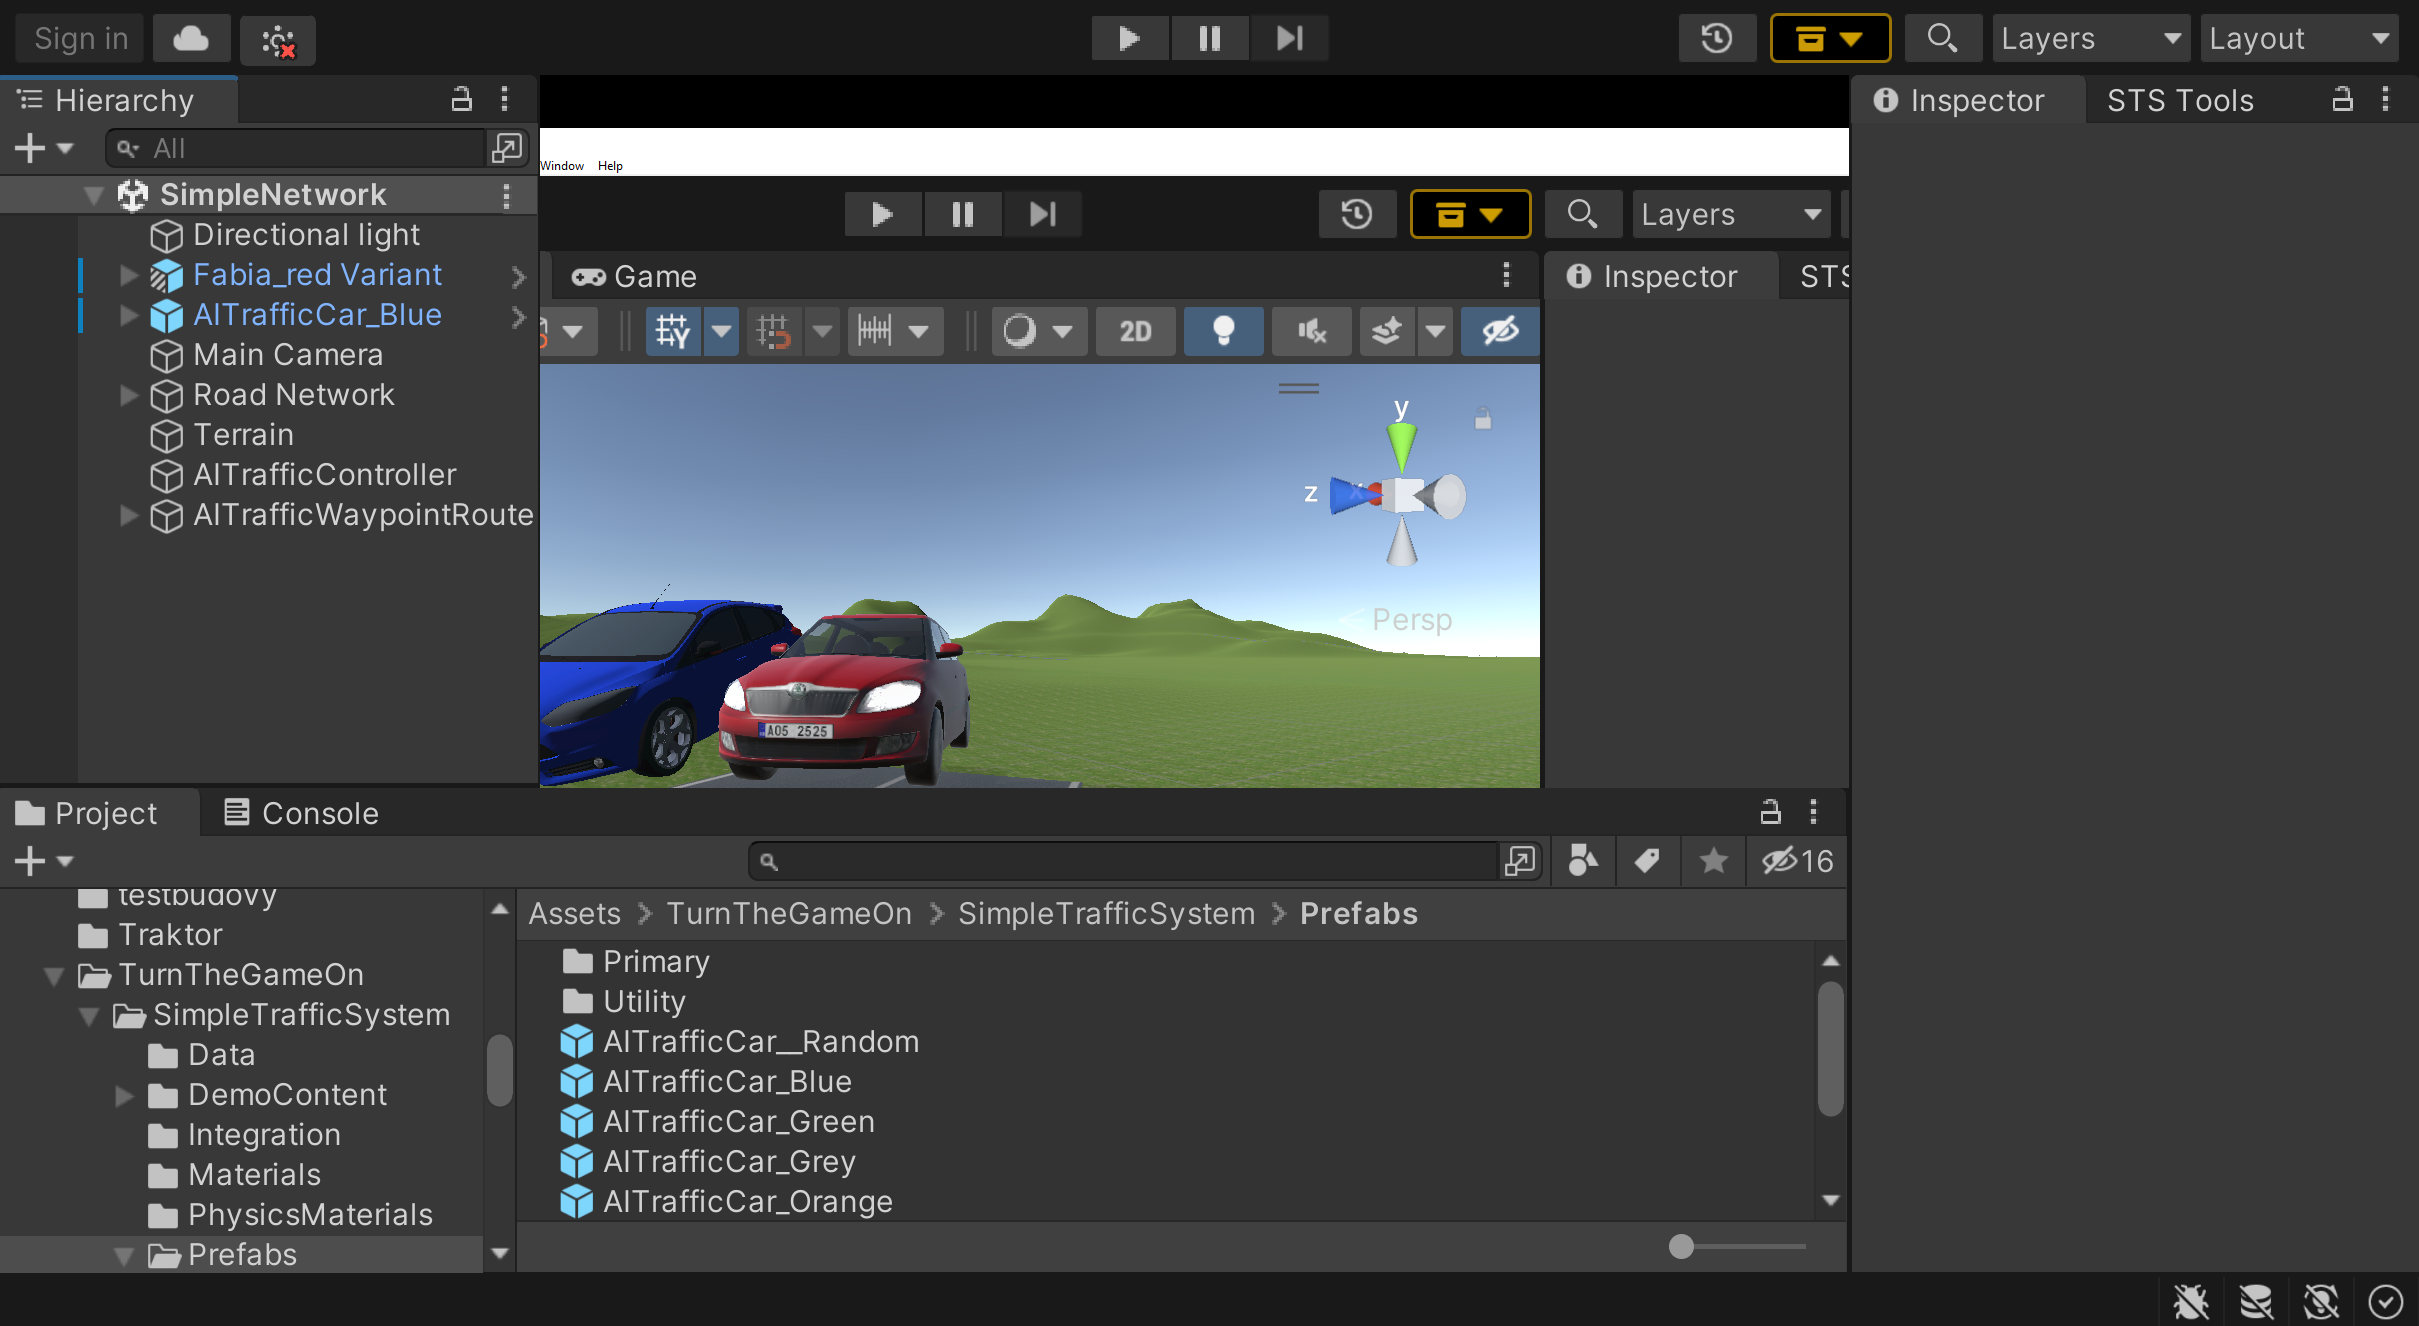
\includegraphics[width=.9\textwidth]{unityUI.png}
    \caption{The Unity development platform UI}
    \label{fig-unity}
\end{figure}

\subsection{Agent Development Platforms}

Having a development tool that is dedicated to agent-based modeling is an advantage as opposed to building the 
system on a "green field", as the tools have the common domain of agent system paradigms implemented and ready 
to use by a designated interface (e.g. communication, localization, state definition), ideally being built in line 
with widespread standards and ideally tested in practical commercial and industrial use. 

An example of popular platforms, according to \cite{Binder2022} can be found below. 

\textbf{JADE} \smallskip \newline 
Jade is a free software developed under a grant from the European Commission. The main advantage of the 
platform is the containerization of agents, which allows to distribute agents across systems, even 
with cross-platform (OS) support. Configuration changes can be done in run-time. The core components of 
the platform are Agent Management System (AMS), Agent Communication Channel (ACC) and Directory Facilitator (DF). 
JADE also supports the FIPA communication standard ACL, mentioned earlier. The platform is implemented with 
the Java programming language.

\textbf{FIPA-OS} \smallskip \newline 
FIPA-OS is an open-source implementation of the FIPA standard. It is a small-footprint development platform, 
which is loosely coupled and offers implementation also on mobile devices. The development is also done 
using Java. 

Although these most popular platforms for agent-based development are industry-tested tools, in the current 
times they are obsolete, as their development was abandoned in the year 2005. Also, most of the 
advantages described, such as multi-platform support and decentralization across machines is not relevant to 
this thesis' use case, as the proposed MAS will be run on one machine, preferably directly within the simulator 
software, to minimize system acceptance conflicts. 

Another issue is that such tools have been developed to run on JVM (Java Virtual Machine), therefore the integration 
with the simulator software would create another layer of complexity to building an ABM framework. 
Related to the system implementation, it is therefore important to choose a platform supporting 
development in C\# language as well, to ensure full and non-complex integration with the simulator 
software.

\textbf{ActressMAS} \smallskip \newline
ActressMAS is a multi-agent framework running on the .NET runtime, written in C\#. The author says that 
its main advantages are conceptual simplicity and ease of use \cite{Leon2022}. The framework's last release was 
in the year 2021, making it a non-outdated option with potentially ongoing development. Notably, the framework is 
open-source, meaning the source code can be inspected and possibly adjusted to the needs of the developed system.

Upon inspecting the source code of ActressMAS, there are three main components that form the basic building 
blocks of a MAS environment - \texttt{Agent}, \texttt{EnvironmentMas} and \texttt{Container}.
The class diagram of the components can be seen in the figure \ref{actress-env} below.

\begin{figure}[htbp]
    \centering
    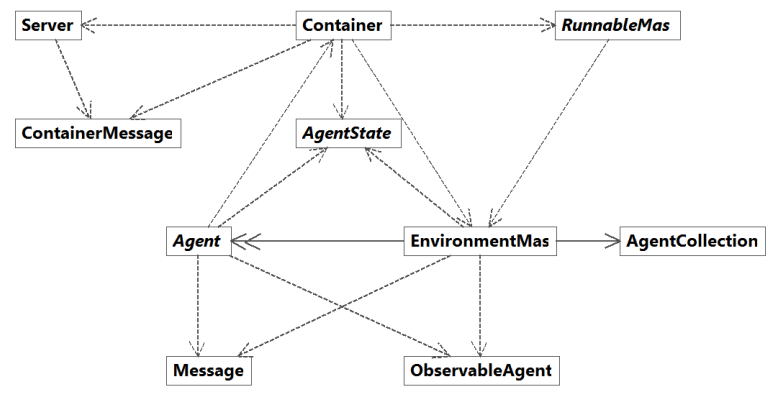
\includegraphics[width=.9\textwidth]{actress-environment2.png}
    \caption{ActressMAS - Class diagram of framework's main components \cite{Leon2022}}
    \label{actress-env}
\end{figure}

The agent environment can be distributed between more machines. Each machine runs a container that communicates with a 
server, as seen in fig. \ref{actress-env}. The service handling communication between containers is a big part of the 
framework, as it is composed of many classes, offering communication through web sockets and even offering to 
use the SSL security protocol and async version of communication, see fig. \ref{actress-distr}.

\begin{figure}[htbp]
    \centering
    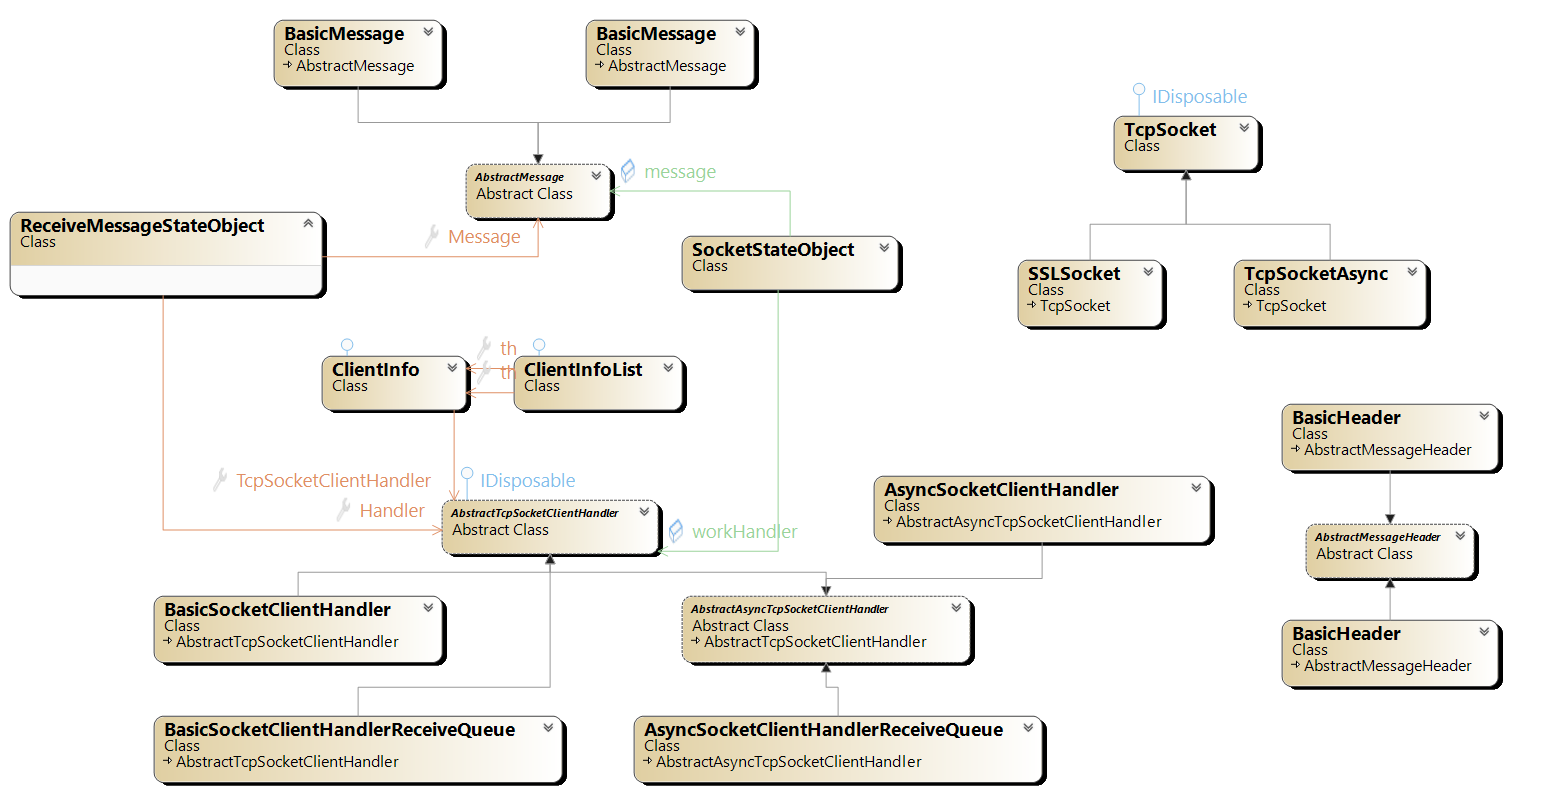
\includegraphics[width=.99\textwidth]{ClassDiagram-actress-containers.png}
    \caption{ActressMAS - Class diagram of distribution service \cite{Leon2022}}
    \label{actress-distr}
\end{figure}

There are, however, some issues related to the use case of the proposed ITS framework. Overall, the implementation of the classes 
creating the local agent environment doesn't contain much (relevant) logic - the logic mostly serves to distribute messages to agents. 
It cannot be clearly said if this is an advantage or a disadvantage, as for specific use-cases, like building an ITS multi-
agent framework is expected to have specialized logic. However, the lack of behavior implementation also means that the 
agent architecture has to be built from the ground up either way, not bringing any benefit to using this framework. 
On a second note, agents only update their state once they receive a message, which doesn't 
meet the requirement for agents to act independently and autonomously. This also means that agents are not able to gather 
and act upon information from their sensors, just from messages received from other agents. This behavior might be implemented 
by the user, but there might be conflicts with the current design of the interaction interface of the agents and the 
\texttt{EnvironmentMas} class that would add redundant effort as opposed to building an agent environment from "scratch". 

\subsection{Conclusion}

In this section, the technical aspects of implementation requirements are discussed. The
simulator engine is introduced, describing the aspects of programming integration. The main
aspects of integration are discussed, which should enhance the subsequent decision about
which MAS development platform to use for the proposed system implementation. Consequently, MAS
development platforms suggested by the literature are examined. However, their review concludes
not to use them as they are outdated and would not offer an advantage concerning integration
with simulator software. Their focus is to integrate with distributed computer networks
focusing on different problems. Lastly, a promising agent-developed framework called 
ActressMAS is introduced, whose main advantage is being .NET/C\# based
and open-source, allowing for adequate customization. However, after further inspection of the
codebase, it was concluded that the way the agent-based system proposed in this thesis is
designed, there were no significant potential benefits that implementation of the framework 
would bring. The ActressMAS framework's implementation revolves around deployment across 
multiple machines and offered minimal abstraction of the agent framework itself, i.e. 
agent behavior and interaction. Therefore, building the framework independent from a
pre-existing MAS platform offers maximum customization according to the system
specification and its requirements. 

\clearpage

\end{document}